% Documento
\documentclass[12pt,a4paper,english,brazil]{article}
    
% Pacotes
\usepackage[utf8]{inputenc}
\usepackage[portuguese]{babel}
\usepackage[T1]{fontenc}
\usepackage[top=2cm,bottom=2cm,left=3cm,right=3cm]{geometry}
\usepackage{amsmath}
\usepackage{graphicx}           % para add imagens
\usepackage{xcolor}             % para usar \textcolor{}{}
\usepackage{float}              % para usar o [H] em imgs
\usepackage[num]{abntex2cite}   % padrão abnt para citação
\usepackage{indentfirst}        % indenta o 1º paragrafo 
\usepackage[colorlinks=true, allcolors=blue]{hyperref}

\begin{document}

% Título ------------------------------------------------------------
\title{ Exercício de Aplicação 4 - Estabilidade de malha de controle \\ 
        SME 301 -  Métodos Numéricos para Engenharia I }
\date{\vspace{-5ex}}
\author{ Monitor João Paulo Casagrande Bertoldo \\
         Prof. Dr. Eduardo Fontoura Costa }
\maketitle
\vspace{15pt}

% Introdução --------------------------------------------------------
\section{Introdução}\label{sec-intro}

No Exercício de Aplicação 3 (dinâmica de uma barra rígida acoplada a um motor de corrente contínua), utilizamos uma técnica amplamente conhecida para a análise de sistemas lineares: os Espaços de Estados. Esta técnica consiste em definir uma variável vetorial cujos elementos são váriáveis representativas do estado de um sistema dinâmico de tal forma que, sabendo seus valores, podemos descrever completamente o sistema (posição, velocidade, aceleração, energia, ...).  \

Porém, um sistema controlado não é composto somente por variáveis internas do sistema; também é preciso levar em consideração as variáveis de entrada do sistema. Estas variáveis são as grandezas que podemos controlar com o objetivo de controlar todo o resto do sistema. \

Em sistemas mecatrônicos e em sistema de automação, colocam-se computadores (analógicos ou digitais) para calcular o comando (\textit{input}) necessário de tal forma que o sistema físico responda da maneira esperada. Em sistemas controlados automaticamente, é comum instalarem-se sensores que fornecem ao computador um sinal elétrico que corresponde a uma medidade física, o que permite que ele consiga calcular o estado em que o sistema se encontra. \

A partir desta informação sobre o sistema, o computador calcula qual deve ser a entrada do sistema para fazê-lo chegar a um estado desejado (por exemplo, fazer o eixo de um motor chegar a uma posição angular desejada). Isto é o \textbf{fechamento de malha} do sistema. \

Uma maneira simples e amplamente utilizada de "fechar a malha" é utilizando um controlador proporcional. O que ele faz é gerar um sinal de entrada (por exemplo, uma tensão $v$) proporcional ao erro da saída real do sistema e o saída desejada (por exemplo, a posição angular medida por um sensor \theta_{medido} e a posição de comando \theta_{comando}). Ou seja, ele calcula uma diferença de sinais e multiplica este resultado por uma constante: $v = K * (\theta_{comando} - \theta_{medido})$. \

Não entraremos em mais detalhes a respeito da teoria de contole, mas perceba que intuitivamente isso faz sentido; quanto mais longe do sinal de comando, maior é a tensão que força o sistema a se mover; da mesma maneira, conforme o sistema se aproxima do estado comandado, a tensão de entrada diminui proporcionalmente. \


% Estabilidade --------------------------------------------------------
\subsection{Estabilidade}\label{sec-estabilidade}

Quando um engenheiro mecatrônico projeta um sistema de controle, é necessário analisar diversos critérios para atender às necessidades do sistema desejado. Por exemplo, pode-se querer que o sistema responda aos comandos:  mais rapidamente; com menos vibração; sem ultrapassar um certo valor de aceleração ou melhorando a resposta a ruídos. \

Um importante aspecto a ser analisado é a \textbf{estabilidade}. Quando se fecha a malha de um sistema (ou seja, criamos um \textit{feedback} da informação de saída para determinar a entrada necessária), o sistema pode tornar-se instável e levar o sistema ao colapso. Para evitar este tipo de problema, podem-se fazer diversas análises de estabilidade utilizando um modelo do sistema real. \

Nesta prática, utilizaremos uma técnica simples de determinação de estabilidade usando a representação em espaço de estados de um modelo. \

% Método --------------------------------------------------------
\subsection{Método}\label{sec-metodo}

Considere que a seguinte equação de espaço de estados:

\begin{equation}
	\pmb{\dot{\mathrm{x}}} \, (t) = A \, \pmb{\mathrm{x}} (t)  + B \, \pmb{u}(t) 
\end{equation}

Onde $\pmb{\mathrm{x}}$ é a variável de estados e $\pmb{u}$ é a variável de comando do sistema.

Para que o sistema seja estável, é suficiente que todos os autovalores da matriz $A$ tenham suas componentes reais negativas (lembrando que os autovalores são complexos). Por exemplo, um sistema com os autovalores da Figura \ref{fig:estavel} é estável, mas o da Figura \ref{fig:instavel} é instável. \

\begin{figure}[H]
\centering
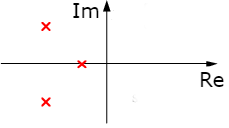
\includegraphics[width=0.7\textwidth]{estavel.png}
\caption{\label{fig:estavel}Exemplo de localização de autovalores de um sistema estável.}
\end{figure}

\begin{figure}[H]
\centering
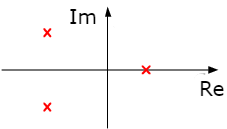
\includegraphics[width=0.7\textwidth]{instavel.png}
\caption{\label{fig:instavel}Exemplo de localização de autovalores de um sistema instável.}
\end{figure}

Porém, não é preciso calcular todos os autovalores do sistema para assegurar que ele seja estável. Basta calcular o autovalor com a maior componente real e verificar se este está à esquerda do eixo imaginário (ou seja, parte real negativa). \

Para isso, vamos utilizar o Método das Potências, que encontra o autovalor de maior \textbf{módulo}. Porém, há um problema: se houverem autovalores com componentes imaginárias, não podemos garantir que o autovalor de maior módulo é também o de maior parte real. \

Vamos contornar este problema fazendo a seguinte operação:

\begin{equation}
	A_{deslocada} = A + k_{deslocamento} * I 
\end{equation}

Onde $k_{deslocamento}$ é um escalar e $I$ é a matriz identidade. Esta operação faz com a matriz $A_{deslocada}$ tenha os mesmos autovalores de $A$ com as componentes reais deslocadas $k_{deslocamento}$ unidades (veja a Figura \ref{fig:deslocamento}). \

Tendo o valor numérico do autovalor de maior módulo da matriz $A_{deslocada}$, basta subtrair $k_{deslocamento}$ deste autovalor para obter o autovalor de $A$ com maior componente real. \

\begin{figure}[H]
\centering
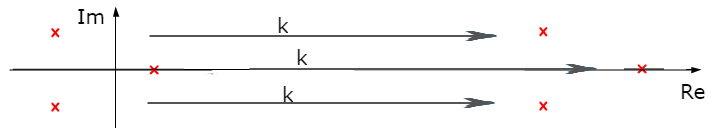
\includegraphics[width=0.7\textwidth]{deslocamento.png}
\caption{\label{fig:deslocamento}Deslocamento dos auto de uma matriz.}
\end{figure}

% Exercício --------------------------------------------------------
\section{Exercício}\label{sec-exer}

O sistema considerado será o mesmo dos Exercícios de Aplicação 2 e 3 e considerando um controlador proporcional. Você deve baixar os scripts neste \href{https://drive.google.com/open?id=0B5SQdylJPM8CYjNXYl92TDR1M1U}{link}, abrir o arquivo "Estabilidade.m" e executá-lo para ver o resultado esperado. \ 

Você deve comentar a linha que faz a chamada do método de referência e descomentar a chamada da função "encontraMaiorAutoValor". Seu código deve ser escrito dentro do arquivo "encontraMaiorAutoValor.m", que é uma função que retorna o autovalor de maior parte real de uma dada matriz $M$ usando o Método das Potências. \ 

A função deve fazer o seguinte:

\begin{enumerate}
	\item Calcular a matriz deslocada $M_{deslocada}$* da matriz de entrada $M$;
	\item Obter seu autovalor de maior módulo usando o Método das Potências;
	\item Calcular o autovalor correspondente da matriz $M$;
\end{enumate}

Obs: o deslocamento deve ser um número "grande" (uma ou duas ordens de grandeza maior do que o determinante de $M$ deve ser suficiente).

\bigskip

Envie seu arquivo de código para \textbf{joao.bertoldo@usp.br} com cópia para \textbf{efcosta@icmc.usp.br} com o assunto "Exercício Adicional 4 - xx", onde "xx" é o seu nome.

\bigskip

\centering{\Large{Boa sorte!}}

\end{document}